\section{Development}

Each component of the project had to be developed individually before assembling them together into a working prototype. The Raspberry Pi, the Sensor Tag and the TelosB. A description of each devices configuration will be described and then how the connection is made between each of them.\\

A good overview of the project can be seen in Figure \ref{fig:over}.

\begin{figure}[!h]
	\begin{center}
		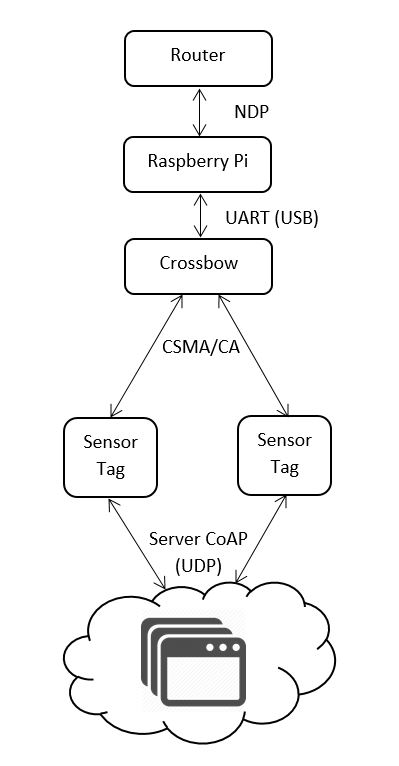
\includegraphics[width=0.6\linewidth]{protocol}
		\caption{sensor node connected with the debugger to a computer}
		\label{fig:over}
	\end{center}
	
\end{figure} 

\subsection{Raspberry pi - 6LoWPAN Boarder Router}

The raspberry pi acts as a boarder router for the WSN in Smart brigde mode (see ). It mitigates information to from the WSN mesh into the IPv6 network of the router. The boarder router is installed into the Raspberry pi via the 6LBR-1.3.3 Packages for Raspian. The service can be started through the terminal and the status of the working service can be seen in Figure \ref{fig:router}.

\begin{lstlisting}[language=bash,caption={start the 6lbr service and check the status}]
$ sudo 6lbr service start
$ sudo service 6lbr status
● 6lbr.service - LSB: 6LoWPAN Border Router
Loaded: loaded (/etc/init.d/6lbr)
Active: active (running); 1h 32min ago
\end{lstlisting}



\begin{figure}[!h]
	\begin{center}
		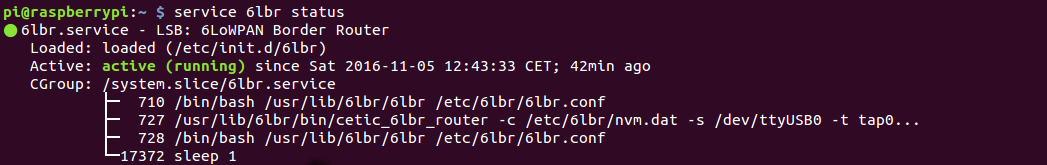
\includegraphics[width=\linewidth]{serviceStatus}
		\caption{The 6lbr service running the boarder router}
		\label{fig:router}
	\end{center}
\end{figure} 

\subsection{TI Sensor Tag - Sensor nodes}



\subsection{Flashing the Texas Instrument Sensor-Tag} 
In order to flash the sensor tag, SmartRF Flash Programmer 2 made by Texas Instrument has been used. For flashing the node a sensor tag needs a Debugger DevPack, the debugger allows for communication to the sensor via USB as it is shown in Figure \ref{fig:debug}.  
\begin{figure}[!h]
	\begin{center}
		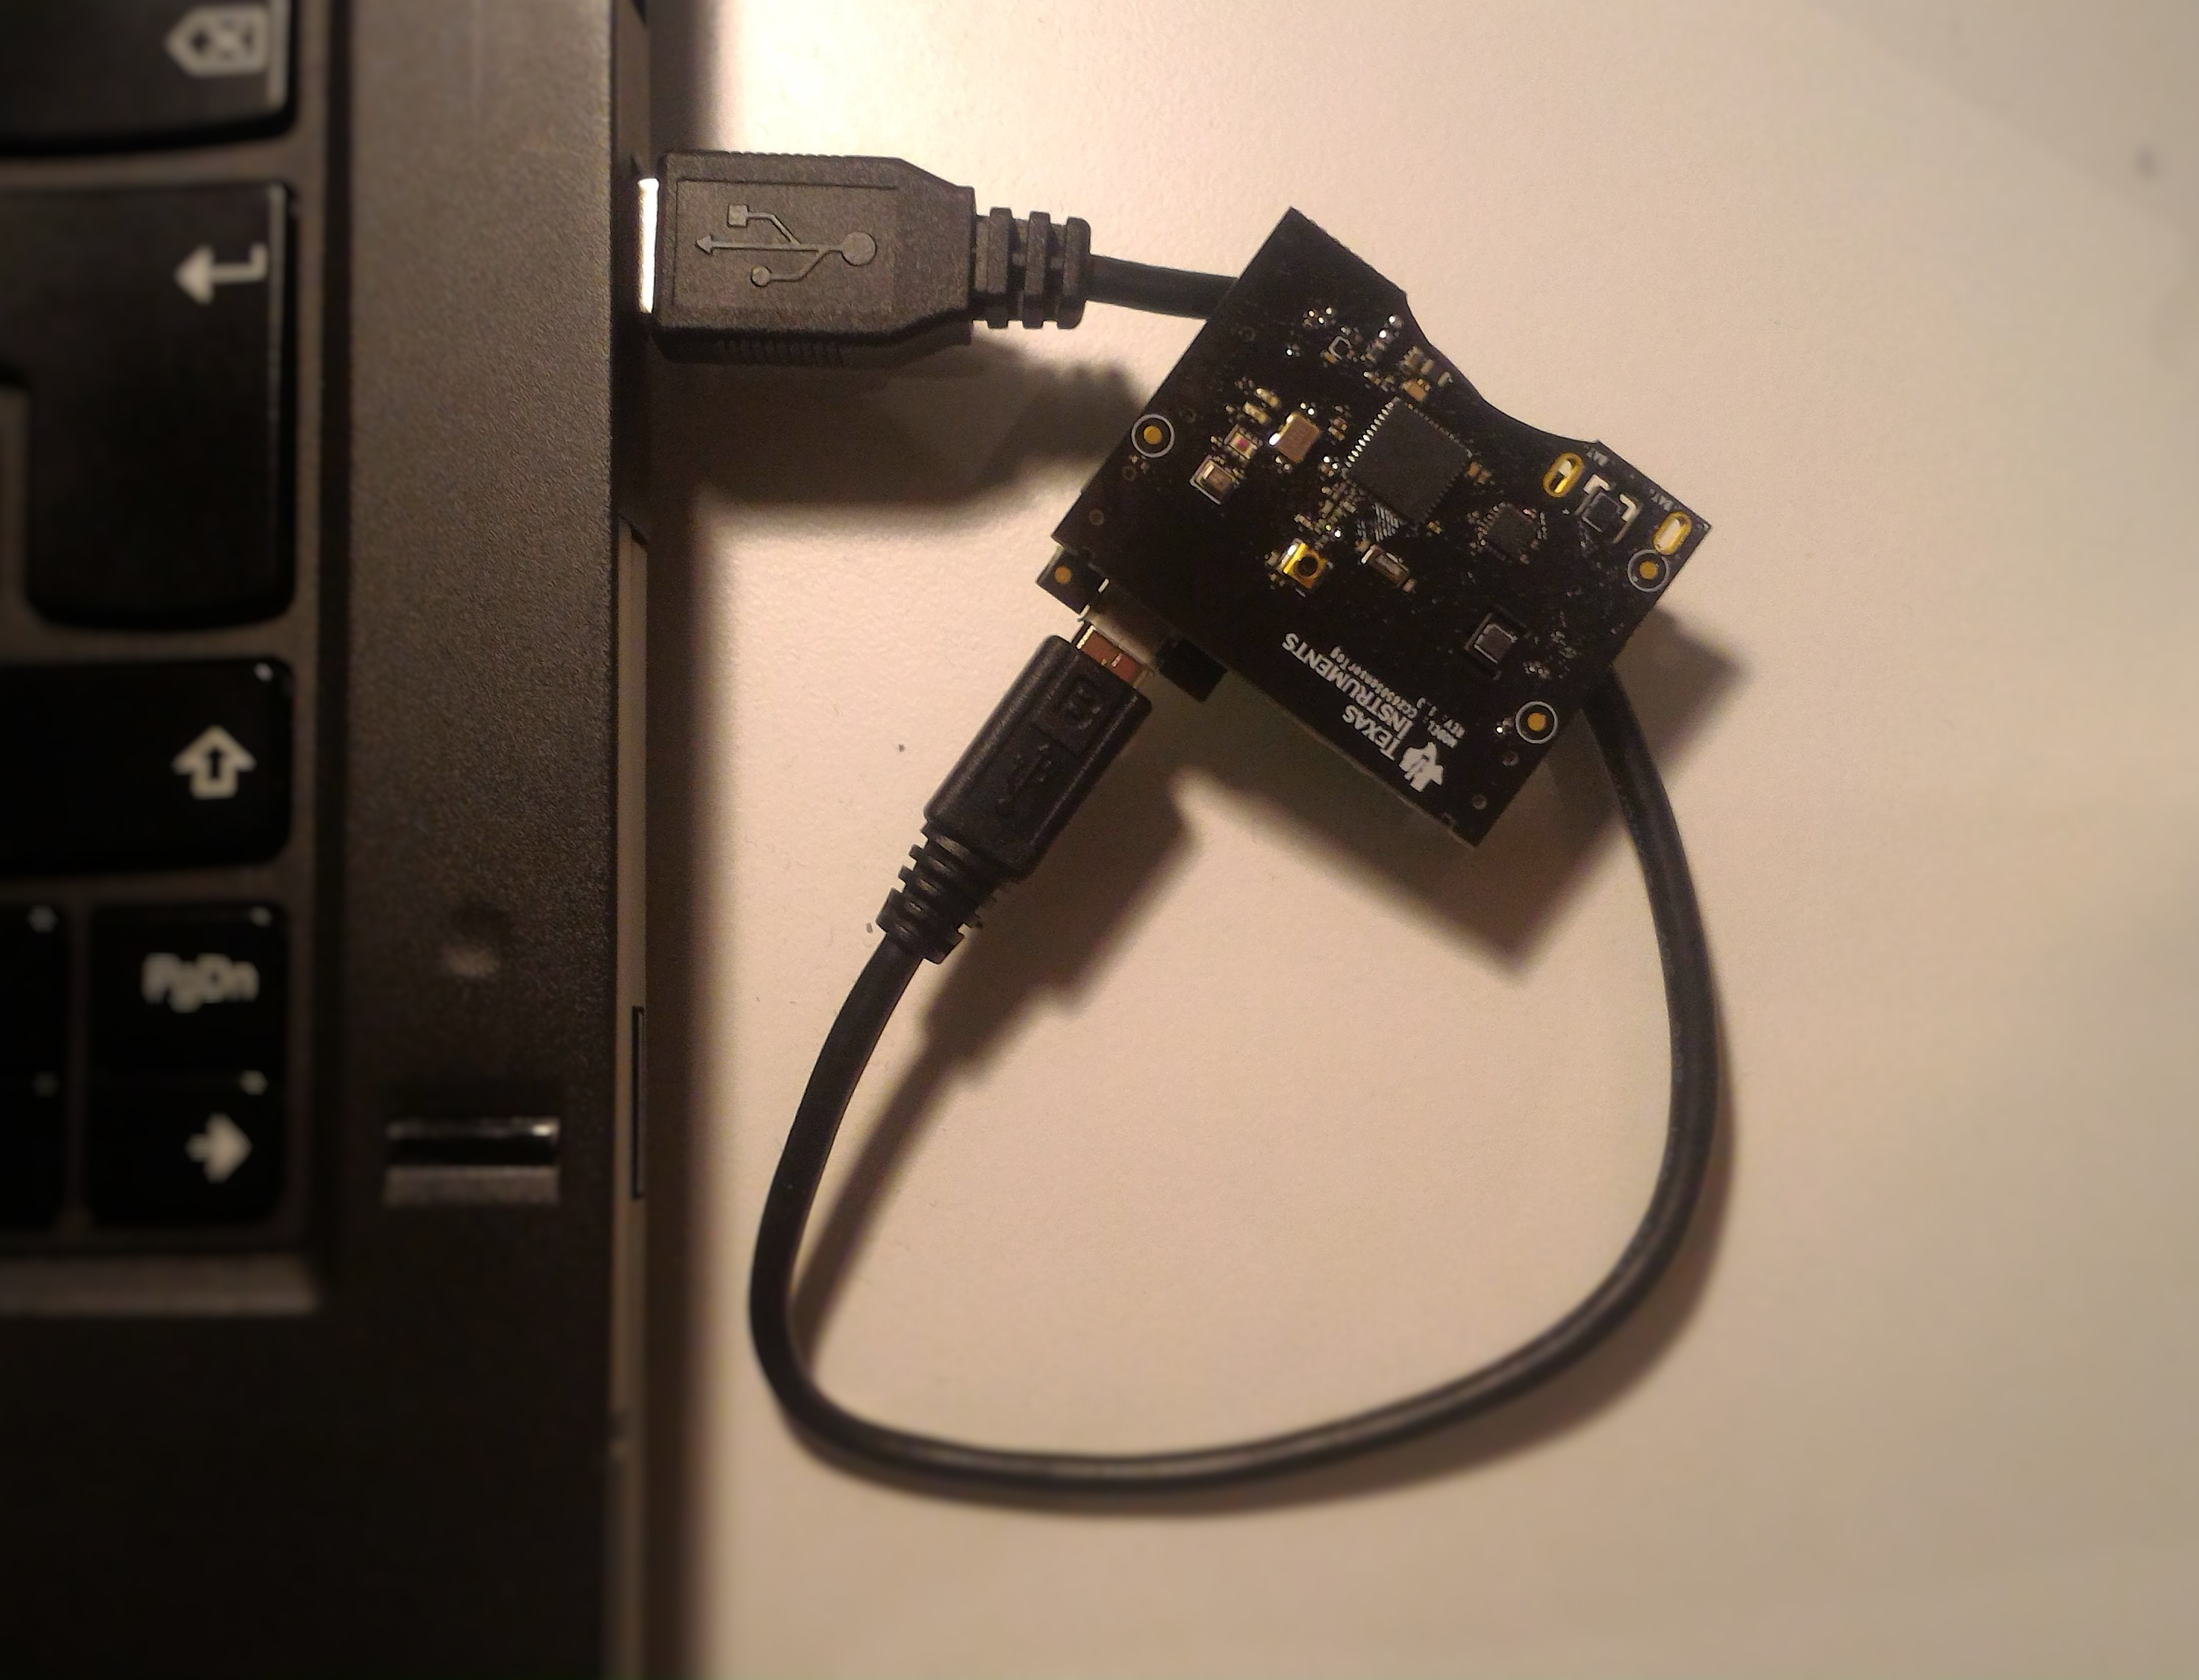
\includegraphics[width=0.8\linewidth]{debugger}
		\caption{sensor node connected with the debugger to a computer}
		\label{fig:debug}
	\end{center}
	
\end{figure} 

\subsection{title}